\makeatletter
\let\@starttocorig\@starttoc
\makeatother

\documentclass[oneside,20pt,fleqn,extrafontsizes]{memoir}

%%% color definition names: xcolor
\usepackage[usenames,dvipsnames]{xcolor}
\definecolor{bulgarianrose}{rgb}{0.28, 0.02, 0.03}
\definecolor{ashgrey}{rgb}{0.7, 0.75, 0.71}
\definecolor{red(ryb)}{rgb}{1.0, 0.15, 0.07}
\definecolor{wocrit}{rgb}{0.75, 0.25, 0.0}

%%% Import other packages%
\usepackage{usepkg}

%% import moodded thing
\usepackage{localF}
\usepackage{mathOp}
%%%%%%%%%%%%%%%%%% refname, titletoc, titlesec setting
\usepackage{titleT-ref}%toc depth

%%%%%%%%%%%% Hyperref package
\usepackage{hyperref}
\hypersetup{
    colorlinks,
    citecolor=black,
    filecolor=black,
    linkcolor=black,
    urlcolor=black
}

%%%%%%%%%%%%%%%%%%%%%%%%
%%%%%%%%%%%%%%%%%Geometry package
\usepackage{mygeometry}
%%%%%%%
\usepackage{fancypkg}%%%import fancy package with memoir correction

%%%%%%%%%%%%%%%%%% setlength
\usepackage{mylength}
\linespread{0.5}

%%%%%%% META
\title{Esami Luglio 19}

%%import makeidx
%\usepackage{makeidx}

%%% COUNTERS
\setsecnumdepth{subsection}
\setcounter{tocdepth}{-1}       % chapter
\newcounter{cherrychapter}%[chapte]
\setcounter{cherrychapter}{1}
\newcounter{partworkouts}%[chapte]
\setcounter{partworkouts}{1}

%%%% iimport functions
\usepackage{functions}
\usepackage{sources}
%%%%%%%%%%%%%%%%%%%% MULTINDExssss (number of chapters)
%\makeindex[1]%biasmomentumoggi]%chapters
%\makeindex[2]%meditazione]
%\makeindex[3]%nitidezza]
%\makeindex[4]%teatro]
\setsecnumdepth{subsection}
\settocdepth{chapter}
 
\begin{document}%BEGIN
\pagestyle{mystyle}%% mystyle defined in usepkg
\renewcommand*{\contentsname}{\label{toc}{Table of Contents}}%%\printcontents without head/hypereff
%\makeatletter
%\renewcommand*{\@tocmaketitle}{\label{toc}{Table of Contents}}
%\makeatother
\maketitle
\startcontents[chapters]

\tableofcontents

\part{Fisica nucleare}
\chapter{BB nucleosynthesis}
\PartialToc

\chapter{Catena PP e ciclo CNO}
\PartialToc

\part{Fundamental interactions}\label{intfon}\label{}{}
\documentclass[main.tex]{subfiles}
 
\begin{document}

\chapter{astro plasma physics}
%\PartialToc

La presenza dello ione $Z_i$ altera la distribuzione di cariche quindi devo determinare il potenziale $\phi_i$ generato da $Z_i$ e dalla distribuzione di cariche attorno; usando la formula di Boltzmann la densit\'a delle particelle con carica Z risulta
\begin{equation}\label{eq:Bdistroelectricpot}
n_Z=\overline{n}_Z\exp{-\frac{Ze\phi}{kT}}
\end{equation}
con $\overline{n}_Z$ densit\'a numerica della particella di carica $Z$ in assenza di $Z_i$.

L'equazione di Poisson per $\phi$ \'e
\begin{equation}\label{eq:poissonscreened}
\nabla^2\phi=-4\pi e\sum_Z Zn_Z-4\pi e\sum_i Z_i\delta(\vec{r}-\vec{r}_i)
\end{equation}

Nel regime di schermaggio debole, dove l'energia coulombiana \'e molto minore dell'energia termica $e\phi\ll KT$, espando $n_Z$ (\eqref{eq:Bdistroelectricpot}) al prim'ordine quindi in \eqref{eq:poissonscreened} rimane il termine lineare in $\phi$.

Introduco il raggio di Debye:
\begin{equation}
\frac{1}{r_D^2}=\frac{4\pi e^2}{kT}\sum Z^2\overline{n}_Z=\frac{4\pi e^2}{kT}N_A\zeta,\ \zeta=\sum_{i}(Z_i^2+Z_i)\frac{\rho X_i}{A_i}\label{eq:debyeradius}
\end{equation}
quindi dall'equazione \eqref{eq:poissonscreened} ottengo il potenziale generato dallo ione $Z_i$ in $\vec{r}_i$ a distanza $|\vec{r}-\vec{r}_i|=r_i$ come soluzione di:
\begin{equation}\label{eq:poissonspheric}
\frac{r_D^2}{r_i}\TtwoDy{r_i}{(r_i\phi_i)}=\phi_i
\end{equation}
con
\begin{equation}
\phi=\sum_i\phi_i
\end{equation}

\begin{workout}[Raggio di debye e degenerazione elettronica]
Il rapporto fra densit\'a elettronica e quella imperturbata \'e
\begin{equation}
\midfrac{f(\psi-\midfrac{U_e(r)}{KT})}{f(\psi)}
\end{equation}
dove $U_e(r)$ \'e l'energia di interazione di un elettrone
\end{workout}

La soluzione di \eqref{eq:poissonspheric} \'e
\begin{equation}\label{eq:screenedpotential}
\phi_i=\frac{Z_ie}{r_i}\exp{-\midfrac{r}{r_D}}
\end{equation}


\chapter{opacity sources}
%\PartialToc

\section{Grain opacity in planetary gas accretion}
$\kappa_{gr}=\frac{Q(x)\pi a^2n_{gr}}{\rho}=\frac{3Q(x)f_{d/g}}{4\rho_{gr}a}$
If $a\gg\lambda$ $Q(x)\approx2$ with $x=2\pi a/\lambda$

\section{ISM dust}
%ism-ch3-dust.pdf
%Dust.pdf
%%vanderanker_slides.pdf
%Draine_IPMU_Lectures.pdf

\chapter{Evapopration ??}
%\PartialToc

Potential
\begin{align*}
&\chi(r)=-\frac{GM_p}{r}+C\\
&\chi'(r)=\chi(r)+\Delta\chi(r)=-G(M_p+M_*)[\frac{\mu}{r}+\frac{1-\mu}{a_p-r}+\frac{((1-\mu)a_p-r)^2}{2a_p^3}]+C\\
&\mu=\frac{M_p}{M_p+M_*}
\end{align*}
Energy needed to escape the planet $\PDy{r}{\chi'}|_{R_h}=0$

\section{Stellar spectrum}

FUV: $\SI{6}{\ev}\leq h\nu\leq\SI{13.6}{\ev}$
EUV: $\SI{13.6}{\ev}\leq h\nu\leq\SI{0.1}{\kilo\ev}$
X-rays: $h\nu\geq\SI{0.1}{\kilo\ev}$

\end{document}

\part{Analisi statistica dati}\label{asd}
disuguaglianza di Chebychev X ha media $\mu$ e var $\sigma^2$ e $\lambda>0$:
\[\prob{(|X-\mu|<\lambda\sigma)}\geq1-\frac{1}{\lambda^2}\]

\documentclass[main.tex]{subfiles}
 
\begin{document}

\chapter{inference}
\PartialToc

\section{Sufficiency}

\subsection{Statistica sufficiente}
\keyword{stat suff}: A statistic T is called sufficient for unknown parameter $\theta$ iff the conditional pdf of iid RV $X_1,\ldots,X_n$ dato $T=t$ don't involve $\theta$. Ex: \iidrv{X} Bernoulli p. $T=\sum_iX_i$ \'e suff: $\prob{(X_1=x_1\cap\ldots\cap X_n=x_n|T=t)}=0$ se $\sum_ix_i\neq t$; $A=\{\cap_iX_i=x_i\}\subseteq B=\{T=t\}$:
\begin{align*}
&\prob{(\cap_iX_i=x_i|T=t)}\\
&=\prob{(\cap_iX_i=x_i\cap T=t)}/\prob{(T=t)}\tag*{P condizionata}\\
&=\prob{(\cap_iX_i=x_i\cap T=t)}/\prob{(T=t)}\tag*{sottoinsieme di $T=t$}\\
&=\prod_i\prob{(X_i=x_i)}/\prob{(T=t)}\tag*{X's independent}
\end{align*}
quindi
\begin{align*}
&\prob{(\cap_iX_i=x_i|T=t)}\\
&=\frac{p\expy{\sum_ix_i}(1-p)\expy{n-\sum_ix_i}}{\binom{n}{t}p^t(1-p)\expy{n-t}}\\
&=1/\binom{n}{t}
\end{align*}
\subsection{T. fattorizzazione Neyman}
iid RV \iidrv{X} pdf $f(x;\theta)$, likelihood $L(\theta)=\prod_if(x_i;\theta)$. $T(X_1,\ldots,X_n)$ \'e suff per $\theta$ iff
\begin{equation*}
L(\theta)=g(T(x_1,\ldots,x_n);\theta)h(x_1,\ldots,x_n)
\end{equation*}
$A=\{X=x\}\subseteq B=\{T(X)=T(x)\}$; only if:
\begin{align*}
&L(\theta)=P_{\theta}(X=x)\\
&=P_{\theta}(X=x\cap T(X)=T(x))\\
&=\underbrace{P_{\theta}(T(X)=T(x))}_{g(T(x_1,\ldots,x_n);\theta)}\underbrace{P_{\theta}(X=x|T(X)=T(x))}_{h(x_1,\ldots,x_n)}
\end{align*}
If part pg 315

\section{Fisher Information}

\subsection{Score statistics}

\begin{align*}
&S=\PDy{\theta}{\log{L}}\\
&\E{[S]}=0\\
&\var{[S]}=-\E{[\PtwoDy{\theta}{\log{L}}]}=-I\\
&S\to N(0,I)
\end{align*}

Informazione di Fisher
\[I_{\Vec{X}}(\theta)=NI_{X_1}=N\E_{\theta}[(\PDy{\theta}\log{f(X_1;\theta)})^2]=-N\E_{\theta}[\PtwoDy{\theta}\log{f(X_1;\theta)}]\]
$I_{X}\geq I_T$ uguaglianza vale per T suff.

\section{Propriet\'a stimatori}

\begin{itemize}
\item consistenza: (LGN) $\E{(\hat{\theta})}\to\theta_0$
\end{itemize}

\section{Stimatori e caratteristiche patametri pdf: gaussian, poissonian, binom - unif}

MVB:

\section{Stimatore MLE di varianza segnale gaussiano con rumore gaussiano}

statistica suff: $s^2=\sum_ix_i^2$
stima mle $\hat{\sigma}^2=\max{(s^2/N-\sigma_0,0)}$.

$Y=\alpha X+b$ $\phi_Y(t)=$

var usando funzione GM della gaussiana
(momento n=2 integrato da $N\sigma_0$
(CRC PRESS 2000, pg 408)

\end{document}

\part{Evoluzione componente solida in dischi protoplanetari}\label{ppd}
\begin{frame}{Accrescimento dei planetesimi: collisioni.}
\begin{itemize}
\item $r_{pl}<b<\frac{Gm_{pl}}{v_r^2}=b_0$: incontro ravvicinato ($|U_{max}|>E_{kin}^{\infty}$ l'energia potenziale nel momento di massima interazione sovrasta energia cinetica a infinito).
\item $b>(\frac{m_{pl}}{3\msun{}})\expy{\frac{1}{3}}a=d_{Hill}$: passaggio a grande distanza.
\item $b_0<b<d_{Hill}$: deflessioni di direzione e verso casuali.
\end{itemize}
\begin{block}{Scattering $b>r_{pl}$: variazione velocit\'a relativa}
\begin{equation*}
\delta v_r=\underbrace{\frac{Gm_{pl}}{b^2}}_{\exv{a}}\underbrace{\frac{2b}{v_r}}_{\exv{\tau_{int}}}=\frac{2Gm_{pl}}{bv_r}
\end{equation*}
\end{block}
\begin{equation*}
b_0<b<d_{Hill}:\quad [\TDy{t}{v_r^2}]_{enc}=\int_{r_{pl}}^d2\pi bv_r\frac{\sigma n}{m_{pl}v_r}(\frac{2Gm_{pl}}{bv_r})^2\,db
\end{equation*}
\begin{block}{Urti anelastici: impatti}
\begin{equation*}
[\TDy{t}{v_r^2}]_{imp}=\pi r_{pl}^2(\frac{\sigma n}{m_{pl}v_r})v_r(-v_r)
\end{equation*}
\end{block}
\end{frame}

\begin{frame}{Accretion rate: collisions with stick prob 1}
\begin{columns}[T]\begin{column}{0.5\textwidth}
\begin{align}
&\TDy{t}{M}=\underbrace{\rho_p}_{n_mm}v_r\pi R^2[1+(\frac{v_e}{v})^2]\\
&\rho_p\approx\frac{\Sigma}{2a\sin{i}}\approx(\frac{\sqrt{3}}{2})(\frac{\Sigma\Omega}{v})
\end{align}
\end{column}\begin{column}{0.5\textwidth}

\end{column}\end{columns}
\end{frame}

\documentclass[main.tex]{subfiles}
 
\begin{document}

\chapter{Newtonian potential}
\PartialToc

\section{two-body}

\section{Hamiltonian}

\begin{align*}
&H(p,q)=\frac{1}{2\mu}(p_r^2+\frac{1}{r^2}p_{\beta}^2+\frac{1}{r^2\cos^2{\beta}}p_{\lambda}^2)-\frac{k^2\mu}{r}
\end{align*}


\section{perturbation}

\section{3-body}

\end{document}

\part{Strutture all'equilibrio idrostatico}\label{stars}
\documentclass[main.tex]{subfiles}
 
\begin{document}

\chapter{stellar model}
%\PartialToc

\section{structure equations} 

\subsection{Dynamical stability}

Una regione stellare \'e convettivamente stabile se una perturbazione di densit\'a infinitesima non cresce ad ampiezza finita.
\begin{align*}
&\rho\PtwoDy{t}{(\Delta r)}=-g\Delta\rho\\
&=-g[\Dcvar{\TDy{r}{\rho}}{e}-\Dcvar{\TDy{r}{\rho}}{amb}]\Delta r
\end{align*}

La forza di Archimede ha verso opposta alla perturbazione se
\begin{equation*}
[\Dcvar{\TDy{r}{\rho}}{e}-\Dcvar{\TDy{r}{\rho}}{amb}]>0
\end{equation*}

\begin{figure}[!ht]
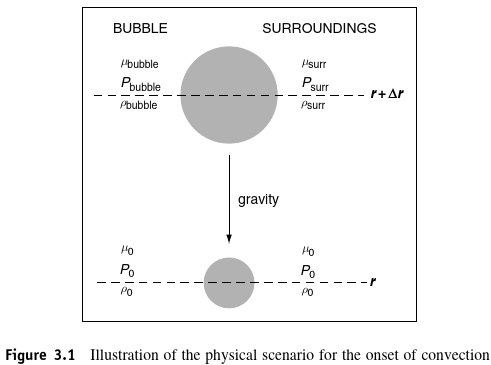
\includegraphics[trim={0cm 0cm 1cm 0cm},clip, keepaspectratio,width=0.99\textwidth]{convectivestability}\label{fig:convectivestability}
\end{figure}

\begin{itemize}
    \item Rayleigh-Taylor instability: $\TDy{r}{\ln{(\mu)}}>0$
    \item $\nrad>\nad-\frac{\xi_{\mu}}{\xi_T}\TDly{(P)}{(\mu)}$
\end{itemize}
		
\subsection{Gradiente ambientale nelle regioni convettive}



\chapter{evolution of stars}
%\PartialToc

\subsection{Massa minima innesco fusione H}

Temperatura minima per innesco idrogeno: $T_{min}\approx\SI{1.5e6}{\kelvin}$
\begin{align*}
&P_c=K_{NR}n_e\expy{5/3}+n_ikT_c=K_{NR}\frac{\rho_c}{m_H}]\expy{5/3}+\frac{\rho_c}{m_H}kT_c\\
&kT_c=A\rho_c\expy{1/3}-B\rho_c\expy{2/3}\\
&kT_{c,max}\propto G^2\frac{m_H\expy{8/3}}{K_{NR}}M\expy{4/3}
\end{align*}

\subsection{Massa massima}

\begin{align*}
&P=P_i+P_e+P_R=\frac{\rho_c}{\mu m_H}kT_c+\frac{1}{3}aT_c^4\\
&P_g=\beta P_c\quad P_R=(1-\beta)P_c
\end{align*}

\subsection{Struttura stellare approssimata}

\begin{itemize}
\item \keyword{Approssimazione zero per $M_r(0)$ e $M_r(R)$}:
Al centro della stella $\TDy{r}{P}=-\frac{GM_r}{r^2}\rho\approx-\frac{4\pi}{3}r^3\rho_c\frac{G}{r^2}\rho_c\approx-\frac{4\pi}{3}rG\rho_c^2$, vicino alla superficie $\TDy{r}{P}\approx-G\frac{M\rho}{r^2}$: se la composizione chimica \'e costante
\begin{align*}
&\TDy{r}{P}\approx-\frac{4\pi}{3}G\rho_c^2r\exp{-r^2/a^2}\\
&P(r)\approx-\frac{2\pi}{3}G\rho_c^2a^2[\exp{-r^2/a^2}-\exp{-R^2/a^2}]
\end{align*}

$4\pi\rho r^2dr=dm$ ci permette di riscrivere equilibrio idrostatico $GM_rdM_r=-4\pi r^4dP$:
\begin{align*}
&\frac{1}{2}GM_r^2=-4\pi\int_0^rr'^4\TDy{r}{P}\,dr\\
&M_r=\frac{4\pi a^3}{3}\rho_c\Phi(x)\quad x=r/a\\
&\Phi(x)=6\int_0^xx'^5\exp{-x'^2}\,dx'\approx x^6-3/4x^8+3/10x\expy{10}+...
\end{align*}
per alta $\rho_x$ $a\ll R$ ...:
\begin{align*}
&M\approx M_r=\frac{4\pi\rho_ca^3}{3}\Phi(\frac{R}{a})\approx\frac{4\pi\rho_ca^3}{3}\sqrt{6}\\
&P_c\approx\frac{2\pi}{3}G\rho_c^2a^2\approx[\frac{\pi}{36}]GM\expy{2/3}\rho_c\expy{4/3}
\end{align*}

\item Politropa $n=3/2$: $P_c\propto M\expy{2/3}\rho_c\expy{4/3}$

\item Politropa $n=3$: $P_c\propto M\expy{2/3}\rho_c\expy{4/3}$

\end{itemize}

\section{Evolution scaling}

\begin{itemize}
    \item \xaumenta{M}, \xdiminuisce{\tau}
    \item \xdiminuisce{M}, \xaumenta{\rho_c}, \xdiminuisce{T_c}
    \item \xaumenta{Z}, \xdiminuisce{L}, \xdiminuisce{T_e}, \xaumenta{\tau}
    \item \xaumenta{Y}, \xaumenta{L}, \xaumenta{T_e}, \xdiminuisce{\tau}
    \item Opacit\'a in funzione di Y: \xaumenta{Y}, \xdiminuisce{\kappa} 
\end{itemize}

\subsection{Low mass star}

tempi evolutivi in HRD


\section{From proto-star to Pre-MS}

\begin{itemize}
\item Isothermal collapse of MC ($t_{cool}\ll t_{ff}$, $P\propto\rho$). MC build up as gas flow into arm's potential well. massa di Jeans $M_J\propto\expy{3/2}\rho\expy{-1/2}$. $M_j$ diminuisce all'aumentare di densit\'a: frammentazione
\item Virial theorem.

\adjm{\rho\TDy{t}{\vec{u}}=-\nabla P-\rho\nabla\phi+\frac{1}{c}\vecp{j}{B}}

\adjm{\rho\TDy{t}{\vec{u}}=-\nabla P-\rho\nabla\phi+\frac{1}{4\pi}(\scap{B}{\nabla})\vec{B}-\frac{1}{8\pi}\nabla|B|^2}

\adjm{\frac{1}{2}\PtwoDy{t}{I}=2T+2U+W+M}

\adjm{I=\int \rho|r|^2\,d^3x,\ T=\frac{1}{2}\int\rho|\vec{u}|^2\,d^3x,\ U=\frac{3}{2}\int nKT\,d^3x=\frac{3}{2}\int P\,d^3x}

\adjm{W=\frac{1}{2}\int\rho\phi\,d^3x\ M=\frac{1}{8\pi}\int|B|^2\,d^3x}

No evidence for collapse of giant complexes: $2T+2U+W+M$.

\adjm{\frac{T}{|W|}\approx\frac{1}{2};\Delta V^2\invers{(\frac{GM^2}{R})}}

\adjm{=0.5(\frac{\Delta V}{\SI{4}{\kilo\meter\per\second}})^2(\frac{M}{10^5\msun{}})\expy{-1}(\frac{R}{\SI{25}{\parsec}})}

\adjm{\Delta V\approx\sqrt{\frac{GM}{R}}=V_{vir},\ t_{ff}\approx\sqrt{\frac{R^3}{GM}}}

Small clumps moving moving in gravitational field of whole ensamble.
\item Denser regions with point IR source. (Fase adiabatica $P\propto\rho\expy{\gamma}$, $T\propto\rho\expy{2/3}$ per mono-ideal gas) Inner region of collapsing cloud becomes denser/optically thicker (first core formation $\tau\approx\SI{1.5e7}{\year}$): role of ambipolar diffusion. Typical mass $M_*=\num{e-2}\msun{}$, $R_*=\SI{5}{\astronomicalunit}$, $\rho\approx\SI{e-10}{\gram\per\cubic\cm}$. Energy radiated by denser core is absorbed by free-falling gas and re-emitted in IR
\item The first core of molecular hydrogen collapse as soon as T is raised enough to begins molecular dissociation (for $T>2000K$ we have collisional diss)
\begin{align*}
&0=-\frac{1}{2}\frac{GM_*^2}{R_*}+\Delta E_{int}+L_{rad}t\\
&L_{rad}\approx L_{acc}=\frac{\dot{M}GM_*}{R_*}\\
&\Delta E_{int}=\frac{XM_*}{m_H}[\frac{\Delta E_{dis}(H)}{2}+\Delta E_{ion}(H)]+\frac{YM_*\Delta E_{ion}(He)}{4m_H}
\end{align*}
\item Birthline
\begin{align*}
&\tau_{KH}=\frac{GM_*^2}{R_*L_*}\propto L_*\expy{-3/2}\\
&\TDy{t}{R_*}\propto-\frac{R_*}{t_{KH}}\\
&L_*=4\pi\sigma T_*^4R_*^2\\
&\TDy{t}{L_*}\propto-\frac{L_*}{\tau_{KH}}
&T_*\approx\const{}
\end{align*}
The most luminous therefore youngest object reflect its nature of accreting object within collapsing dense core: surface temperature and luminosity are set by infall (\numrange{e-5}{e-6}$\msun/yr$) dynamics (expected to change when infall end), radius by internal structure and is the same for protostar and pre-MS star; the birthline is the locus of pre-MS star with protostellar radii. At $M_*=8\msun$ the birthline intercept the ZAMS
\item Slower accretion give radius more time to shrink but D-burning thermostat limit that. D ignition: $^2H+^1H\to^3He+\gamma(\SI{5.5}{\mega\ev})$.
\item ''position'' of Hayashi track: \xaumenta{Y}, \xaumenta{T_e}; \xaumenta{Z}, \xdiminuisce{T_e}; \xdiminuisce{M}, \xdiminuisce{T_e}
\item formation of radiative core caused by \xdiminuisce{R}, \xdiminuisce{L}, \xdiminuisce{\nabla_{rad}} ($L\propto R^2$); parallelamente \xdiminuisce{R}, \xaumenta{T}, \xdiminuisce{\exv{\kappa}} ($\kappa_{kr}\propto$), \xdiminuisce{\nrad{}}, \xaumenta{T_e}
(stahler palla fig 16.8)
\end{itemize}

\subsection{Pre-MS star model}
Structure equation:
\begin{align*}
&\PDy{M_r}{r}=\frac{1}{4\pi r^2\rho}\\
&\PDy{M_r}{P}=-\frac{GM_r}{4\pi r^4}\\
&\PDy{M_r}{L_{int}}=\epsilon-T\PDy{t}{s}
\end{align*}
fourth equation in radiative/convective zones
\begin{align*}
&T^3\PDy{M_r}{T}=-\frac{3\kappa L_{int}}{256\pi^2\sigma r^4}\\
&\PDy{M_r}{s}
\end{align*}
HE integrated from phot to inf
\adjm{P_{phot}=\frac{GM_*}{R_*^2}\int_{R_*}^{\infty}\rho\,dr\approx\frac{GM_*}{R_*^2\kappa_{phot}}\int_{R_*}^{\infty}\rho\kappa\,dr=\frac{GM_*\Delta\tau}{R_*^2\kappa_{phot}}}
(adim eqs:
\adjm{x=\frac{r}{R},\ q=\frac{M_r}{M},\ t=\frac{T}{T_0},\ p=\frac{P}{P_0},\ T_0=\frac{\mu GMm_H}{Rk},\ P_0=\frac{GM^2}{4\pi R^4}}
Continuity: $\TDy{x}{q}=\frac{p}{t}x^2$, HE: $\TDy{x}{p}=-\frac{p}{t}\frac{q}{x^2}$, $\nad$ for fully convective star: $P=CT\expy{5/2}\to p=Et\expy{2.5}$ (C determines the adiabat).
HayT is vertical $\TDly{T_e}{L}>10$, mild mass deps $\TDly{M}{T_e}\approx0.2$. Realistically: surface condition+super-adibat layer.
)

As T increses due to contraction (V.T.)a central radiative core is formed: when a sizeble radiative core formed path toward higher $T_e$ is almost horizontal.
At temperature \SIrange{1e6}{2.5e6}{\kelvin} D/Li(Be/B) are burnt by proton capture (Li/D depletion at surface for fully convective star).
In general larger masses have lower Li depletion, given mass increases increasing Z: \xaumenta{M}(or \xdiminuisce{Z}) lower convective zone but also earlier retreat from center (fig 16.10)


\section{Sequenza principale}

\section{From H central exhaustion to He central ignition: overall contraction/TO to TRGB}

\subsection{Low mass stars ($M_{cSC}\approx0.1\msun$)}

\begin{itemize}
\item As H exhausts in center $T_M$ moves outward: at TO $90\%$ of H-burning in thick shell of $0.2\msun$: H-burning shell becomes thinner and thinner as CNO is strongly T-dep and as H-depleted inside and T drops in envelope.
\end{itemize} 

\end{document}

\stopcontents[chapters]
\end{document}